\chapter{GİRİŞ}\label{CH1}
Python Görüntü İşleme kütüphaneleri ile gerçek zamanlı görüntü işlemeleri yapılabileceği gibi analizleri de gerçekleştirilir.
\\
Görüntü işleme, genellikle estetik bir standart elde etmek veya tercih edilen bir gerçekliği desteklemek için bir görüntüyü keyfi olarak manipüle etmek olarak görülür. Bununla birlikte, görüntü işleme, insan görsel sistemi ile dijital görüntüleme cihazları arasında bir çeviri aracı olarak daha doğru bir şekilde tanımlanır.
\\
İnsan görsel sistemi, ek gürültü ve bant genişliği kısıtlamaları getiren görüntüleme cihazlarıyla dünyayı dijital dedektörlerle aynı şekilde algılamaz. İnsan ve dijital detektörler arasındaki göze çarpan farklar, çeviriyi gerçekleştirmek için bazı temel işlem adımlarıyla birlikte gösterilecektir.
\\
Görüntü işlemeye bilimsel yöntemle tutarlı bir şekilde yaklaşılmalıdır, böylece diğerleri yeniden üretebilir ve birinin sonuçlarını doğrulayabilir. Buna, işleme eylemlerinin kaydedilmesi ve raporlanması ve benzer tedavilerin yeterli kontrol görüntülerine uygulanması dahildir.
\\
Böylelikle elde edilen görüntünün anlaşılabilirliği ,verimliliği ve çözünürlüğü en üst kalitede çıktı olarak elimize geçer.
Görüntü işleme kütüphanelerinin izlediği yöntemler ve algoritmalarının taşıtlar üzerinde kullanılıp plaka tanımlamalarının yapılabilmesi hedeflenir.\\
Plakalar tanımlandıktan sonra proje içerisinde hedeflenilen, araçların otopark ücretleri ve otoparktaki konum bilgilerine erişilir.
\section{Tezin Amacı}
Python Görüntü İşleme Kütüphaneleri aracılığıyla bir otoparka giriş yapacak olan taşıtların gerçek zamanlı plaka görüntüleri saptanır ve bellekte tutulur. Hafızada tutulan taşıt plakalarına göre, her taşıtın park yeri konum bilgilendirmesi elde edilir. Otoparkta taşıtların kalma sürelerine ilişkin veriler, plakalarına bağlı olarak bellekte saklanır.Böylelikle her plakaya ait otopark ücreti ve otoparkta hangi konuma park edildiğini otomatik olarak öğrenebilmek amaçlanır.Otoparkı bulunan işletmelerde park ücretinin sistem üzerinden otomatik olarak hesaplanması hedeflenir. Hayatın günlük karmaşasında insanoğlu unutkanlık yaşayabileceği gibi aracını park ettiği katı veya bloğu otopark içerisinde unutabilir. Bu projede aracımızın otopark konum bilgisi kolaylıkla elde edilir.
\section{Görüntü İşleme Neden Önemlidir?}
\cite{görüntüişleme}Görüntü İşleme,  elimizde bulunan görüntüden anlamlı ifadeler çıkarmamıza yarayan işlemler bütünüdür. Bu işlemler, görüntüyü oluşturan pikseller üzerinde gerçekleştirilecek matematiksel işlemler sayesinde gerçekleştirilir. Görüntü elde edildikten sonra, yapılması istenen göreve göre bir algoritma tasarlanır ve görüntü bu aşamalardan geçerek istenen görevi yerine getirir.
Görüntü işleme teknikleri kullanılarak yapılabilecek işlemlere göz atacak olursak şunları görebiliriz;
\begin{itemize}
\item Görüntü üzerinde bulunan gürültülerin arındırılması ve temiz bir görüntü elde edilmesi
\item Görüntü üzerinde bulunan ve insan algısının görmekte zorlandığı nesnelerin tespiti
\item Görüntünün daha kaliteli bir hale getirilmesi
\item Nesne takibi yapılması
\item Görüntü üzerindeki farklı nesnelerin birbirinden ayırt edilmesi
\end{itemize}

\begin{figure}
    \centering
    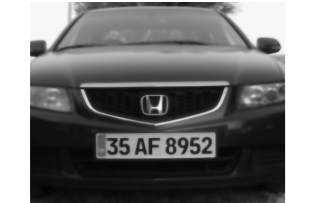
\includegraphics{biteral filtre.PNG}
    \caption{Görüntü işleme ile Araç plakası tanıma }
    \label{fig:my_label}
\end{figure}
\section {Görüntü İşlemenin Kullanım Alanları Nelerdir?}
\newpage
\subsection{Görüntü İyileştirme}
Alınan görüntülerde gürültü olarak adlandırılan ve görüntü üzerinde bozulmalara neden olan bazı istenmeyen yapılar bulunabilir. Bu gürültülere örnek olarak tuz-biber gürültüsü, gauss gürültüsü, shot gürültüsü verilebilir. Görüntü işleme teknikleri içerisinde bulunan mean (ortalama) filtre, medium (ortanca) filtre gibi tekniklerle görüntü daha kaliteli ve gürültüsüz hale getirilebilir. Bu sayede görüntü üzerinde daha doğru sonuçlar elde edilecektir.
\subsection{Cisim Tanıma}
Tespit edilecek cisme göre gerekli yöntemler ve algoritmalar kullanılarak görüntü üzerinden herhangi bir cismin tespiti ve takibi gerçekleştirilebilir. Örneğin yurt dışında  bir çok ülkede suçluların tespiti bu yöntem ile gerçekleştirilmektedir. Mevcut olan kamera düzeneklerinden alınan görüntüler üzerinden her hangi bir insanın tespiti sağlanabilir. Bunun dışında trafik alanında da kullanımı mevcuttur. Trafik içerisinde bulunan araçları sayabilir ve araçların hızı ölçülebilir. Bu sayede trafik yoğunluğu olma ve ya aşırı hız yapma gibi durumların tespiti gerçekleştirilip merkeze gerekli bildirimler yapılabilir.
\subsection{Sağlık Sektörü}
Görüntü işleme teknikleri sayesinde bir çok hastalığın teşhisi gerçekleştirilebilmektedir. Doğum öncesi fetüsün oluşumu ve takibi, tıbbi görüntülerin incelenmesi ,şüpheli dokuların belirgin hale getirilip uzmanlara doğru tanı koyabilme olanağı tanıması, meme kanserinin erken teşhisi gibi alanlarda görüntü işleme teknikleri kullanılmaktadır. Bunların yanı sıra beyin görüntüleme, kemik şeklinin ve yapısının analizi, kanser tanısı koyma ve tümörü fark etme gibi işlemlerde tıp biliminde kullanılabilmektedir.
\subsection{Savunma Sanayi}
İnsansız hava araçları, görüntü ile hedef takibi yapan roketler gibi araçların bünyesinde bulunan donanımlar, görüntü işleme sonucu elde edilen veriler doğrultusunda hareket gerçekleştirir.
\subsection{Diğer Kullanım Alanları}
Diğer alanlardan bazıları ise şu şekildedir;
Uydu görüntüleri üzerinden nüfus yoğunluğu, çevre kirliliği gibi çevresel durumların tespiti,
Hava Gözlem Ve Tahmin,
Güvenlik Sistemleri,
Kriminal Laboratuvarlar,
Uzaktan Algılama Sistemleri.\\
\newpage

\section{LİTERATÜR TARAMASI}

Anıl Güngördü - Araç Plaka Tanıma Sistemi(Verileri tanıtmak için bir xml dosyası oluşturmuştur.Bu xml dosyası 3 exe den meydana gelmektedir.Annotation.exe, createsamples.exe, traincascade.exe’dir. Verileri eğitme aşamaları anlatılmaktadır.)  
\\ \\
Nisanur Bulut - Plaka Tanıma (Bu projede benim projemden farklı olarak araç plakası tanınması sırasında Aforge Kütüphanesi ve Damla Filtreleme İşlemi uygulanmıştır.)  
\\ \\
Neeramitra Reddy - Digital Image Processing(Dijital görüntü işleme aşamalarından, bu aşamaların gerekliliklerinden, dijital görüntü işleme kavramının ne olduğundan , faydalarından ve kullanım alanlarından bahsedilmiştir.)
\\ \\
Rohit Kumar Jena -Automatic Watermark Detection (Dijital görüntü işleme projesidir. Otomatik filigran algılama anlamına gelir.Projede dijital damgalama yaşam döngüsü aşamaları kullanılmıştır.)
\\ \\
Data Carpentry - Image Processing(Skimage'de görüntü temsiline, çizim ve bitsel işlemlere, histogram oluşturmaya, resimleri bulanıklaştırmaya,eşik işlemlerine ve son olarak da bağlı bileşen analizine dair bilgilere yer verilmiştir.) 
\\ \\
Muhammed Mücahid Enes YÜCEL- Görüntü İşleme ile Araç Takibi (Python'da OpenCv kütüphanesi içerisinden çekilen fonksiyonlar kullanılmıştır. Uygulamada görüntü işleme teknikleri ile araç takibi yapıp sonrasında araç sayısı gösterilerek proje gerçekleştiriliyor.)
\\ \\
Bhanu Prakash Poluparthi - Image Processing with Python (Python görüntü işleme kütüphaneleri kullanılmıştır.Görüntü işlemenin ek olarak; komşuluk işlemesine(neighbourhood processing) , segmentasyon analizine, çekirdek dışı görüntü işlemesine , renk manipülasyonuna değinilmiştir.)
\\ \\
Hasaan Majeed-Number Plate Recognition System Using OpenCV (Python'da OpenCV kullanılarak yapılan araç plaka tanıma sistemidir. Görüntüden olduğu kadar videodan da plaka algılamak için kullanılabilecek bir projedir.)
\\ \\
Barroso J., Rafael A.,. Dagless E. L and BulasCruz J.-Number plate reading using computer vision, IEEE Barroso J., Rafael A.,Dagless E. L and BulasCruz J.(Bir plaka tanıma sistemi projesi yaparak görüntüdeki plaka alanının konumu, karakterlerin segmentasyonu ve karakterlerin tanımlanması gereçekleştirilir.)
\\ \\
Gonzalez R. and Woods R. - Morphology-based
License Plate Detection from Complex Scenes(Bu proje, karmaşık sahnelerden renkli kenar kullanan bir plaka algılama algoritması sunmaktadır. Önerilen yöntem dört adıma ayrılabilir:orijinal görüntüden dikey renk kenarı elde etmek, yatay adaylar elde etmek,dikey ve yatay renk kenarlarını içeren LP'nin renk kenarını elde etmek,doğru satır ve çizgi konumlarını bulmak.)
\\ \\
Christos-Nikolaos E. Anagnostopoulos; Ioannis E. Anagnostopoulos; Ioannis D. Psoroulas-License Plate Recognition From Still Images and Video Sequences: A Survey (Görüntülerdeki veya videolardaki plaka tanıma (LPR) algoritmaları plaka formatlarının çeşitliliği ve görüntü elde etme sırasındaki eşit olmayan dış aydınlatma koşulları nedeniyle oldukça zordur. Hareketsiz görüntülerde veya video dizilerinde LPR için çok sayıda teknik geliştirilmiştir ve bu makalenin amacı bunları sınıflandırmak ve değerlendirmektir.)
\\ \\
B. Y. Amirgaliyev; C. A. Kenshimov; K. K. Kuatov; M. Z. Kairanbay; Z. Y. Baibatyr - License plate verification method for automatic license plate recognition systems (Otomatik plaka tanıma (ALPR), insan etkileşimi olmadan bir video akışından veya bir görüntüden plaka numaralarının tanımlanması için kullanılan teknolojidir. ALPR, kayıt veya muhasebe (ücretli yollar, kontrol noktaları ve otoparklar), arama ve takip (çalınan araçların kurtarılması, suçluların yakalanması ve trafik kanunlarının diğer düzenlemeleri) vb. gibi birçok uygulamaya sahiptir.)
\\ \\
Zhuang Liu; Yuanping Zhu - Vehicle License Plate Recognition In Complex Scenes (Bu makale, karmaşık arka plan ve plaka eğimi altında plaka tanıma problemini incelemektedir. Mevcut yöntemler bu sorunları iyi çözemez. Bu makale, derin öğrenmeye dayalı uçtan uca bir düzeltme ağı önermektedir. Model üç bölümden oluşmaktadır: Plaka düzeltme, görüntü özelliği çıkarma ve plaka karakter tanımanın bozulmasından sorumlu olan düzeltme ağı, artık modül ve sıra modülü.)
 \\ \\
 



\newpage

